% XeLaTex
%\documentclass[review]{cvpr}
\documentclass[final]{cvpr}

\usepackage[UTF8]{ctex}

%\usepackage{cvpr}
\usepackage{times}
\usepackage{epsfig}
\usepackage{graphicx}
\usepackage{amsmath}
\usepackage{amssymb}
\usepackage{subfigure}
\usepackage{overpic}

\usepackage{enumitem}
\setenumerate[1]{itemsep=0pt,partopsep=0pt,parsep=\parskip,topsep=5pt}
\setitemize[1]{itemsep=0pt,partopsep=0pt,parsep=\parskip,topsep=5pt}
\setdescription{itemsep=0pt,partopsep=0pt,parsep=\parskip,topsep=5pt}


\usepackage[pagebackref=true,breaklinks=true,colorlinks,bookmarks=false]{hyperref}

% 伪代码
% \usepackage[linesnumbered,ruled]{algorithm2e}
\usepackage{algorithm}
\usepackage{algpseudocode}
\renewcommand{\algorithmicrequire}{\textbf{Input:}}  % Use Input in the format of Algorithm
\renewcommand{\algorithmicensure}{\textbf{Initialization:}} % Use Output in the format of Algorithm

%\cvprfinalcopy % *** Uncomment this line for the final submission

\def\cvprPaperID{159} % *** Enter the CVPR Paper ID here
\def\confYear{ICML 2021}
\def\httilde{\mbox{\tt\raisebox{-.5ex}{\symbol{126}}}}

\newcommand{\cmm}[1]{\textcolor[rgb]{0,0.6,0}{CMM: #1}}
\newcommand{\todo}[1]{{\textcolor{red}{\bf [#1]}}}
\newcommand{\alert}[1]{\textcolor[rgb]{.6,0,0}{#1}}

\newcommand{\IT}{IT\cite{98pami/Itti}}
\newcommand{\MZ}{MZ\cite{03ACMMM/Ma_Contrast-based}}
\newcommand{\GB}{GB\cite{conf/nips/HarelKP06}}
\newcommand{\SR}{SR\cite{07cvpr/hou_SpectralResidual}}
\newcommand{\FT}{FT\cite{09cvpr/Achanta_FTSaliency}}
\newcommand{\CA}{CA\cite{10cvpr/goferman_context}}
\newcommand{\LC}{LC\cite{06acmmm/ZhaiS_spatiotemporal}}
\newcommand{\AC}{AC\cite{08cvs/achanta_salient}}
\newcommand{\HC}{HC-maps }
\newcommand{\RC}{RC-maps }
\newcommand{\Lab}{$L^*a^*b^*$}
\newcommand{\mypara}[1]{\paragraph{#1.}}

\graphicspath{{figures/}}

% Pages are numbered in submission mode, and unnumbered in camera-ready
%\ifcvprfinal\pagestyle{empty}\fi
%\setcounter{page}{409}

%\usepackage{fancyhdr}
%\chead{header}

\begin{document}
% \begin{CJK*}{GBK}{song}

\renewcommand{\figref}[1]{图\ref{#1}}
\renewcommand{\tabref}[1]{表\ref{#1}}
\renewcommand{\equref}[1]{式\ref{#1}}
\renewcommand{\secref}[1]{第\ref{#1}节}
\def\abstract{\centerline{\large\bf 摘要} \vspace*{12pt} \it}

%%%%%%%%% TITLE

\title{
	%\rule{\linewidth}{1.0mm}\\[0.4cm]
	基于子图探索的图神经网络可解释性研究\thanks{本文为ICML'21论文
\cite{yuan2021explainability}的中文翻译版。}
	%\rule{\linewidth}{0.5mm}
	}

\author{Hao Yuan$^{1}$\quad Haiyang Yu$^{1}$ \quad Jie Wang$^{2}$
    \quad Kang Li$^{3}$  \quad Shuiwang Ji$^{3}$  \\
    $^{1}$ Texas A\&M University \quad \quad
    $^2$  University of Science and Technology of
    China \\ $^3$ West China Biomedical Big Data Center\\
    由杨文韬 18020100245 进行翻译与 \LaTeX 重排
}

\maketitle
% \thispagestyle{empty}

%%%%%%%%% ABSTRACT
\begin{abstract}
我们考虑图神经网络 (graph neural networks, GNN) 预测的可解释性问题,该问题被认为是黑盒。现有的方法总是侧重于解释图节点或边的重要性,而忽略了更直观、更容易理解的图的子结构。在这项工作中,我们提出了一种新的方法,称为 SubgraphX,通过识别重要的子图来解释 GNN。给定一个训练好的 GNN 模型和一个输入图,我们的 SubgraphX 可以通过蒙特卡洛树搜索法有效地探索不同子图来解释它的预测。为了使树搜索更有效,我们建议使用Shapley值作为子图重要性的度量,它也可以捕获不同子图之间的交互。为了加快计算速度,我们提出了计算图数据 Shapley 值的有效近似方案。我们的工作首次尝试通过明确和直接地识别子图来解释 GNN。实验结果表明,我们的 SubgraphX 在保持计算在合理水平的同时,实现了显著的可解释性改进。
\end{abstract}



%%%%%%%%% BODY TEXT %%%%%%%%%%%%%%%%%%%%%%%%%%%%%%%%%%%%%%%%
\section{引言}\label{sec:Introduction}

图神经网络由于在各种图任务(包括图分类、节点分类、链接预测和图生成)上具有良好的性能,近年来受到了广泛的关注。人们已经提出了不同的技术来提高深度图模型的性能,例如图卷积和图池化。然而,这些模型仍然被视为黑盒,它们的预测缺乏解释。如果不理解和推理预测背后的关系,这些模型就不能被理解和完全信任,这就阻碍了它们在关键领域的应用。这就需要研究深图模型的可解释性。

最近,人们对图像和文本的深度模型的解释技术进行了广泛的研究。这些方法可以通过不同的策略解释一般的网络行为和特定的输入预测。然而,关于 GNN 的可解释性研究还较少。与图像和文本不同,图表不是类似网格的数据,它包含重要的结构信息。因此,图像和文本的方法不能直接应用。虽然最近的一些研究开发了 GNN 解释方法,如 GNNExplainer,PGExplainer 和 PGM-Explainer ,他们总是专注于节点、边缘或节点特征级别的可解释性,只通过正则化项间接考虑子图。我们认为子图级别的解释更直观和有用,因为子图可以是复杂图的简单构建块,并且与图的功能高度相关。

在这项工作中,我们提出了一种新的 GNN 解释方法 SubgraphX,它可以识别重要的子图来解释 GNN 预测。具体来说,我们建议使用蒙特卡洛树搜索算法来有效地探索给定输入图的不同子图。由于 GNN 中的信息聚合过程可以被解释为不同图结构之间的交互作用,我们建议使用 Shapley 值通过捕捉这种交互作用来衡量子图的重要性。此外,通过只考虑信息聚集范围内的交互作用,我们提出了对 Shapley 值的有效逼近方案。总之,我们的工作代表了通过明确识别子图来解释 GNN 的第一次尝试。我们进行定性和定量实验来评估我们的 SubgraphX 的有效性和效率。

实验结果表明,我们提出的SubgraphX可以更好地解释各种GNN模型。此外,我们的方法由于其优越的性能,具有合理的计算成本。

%%%%%%%%%%%%%%%%%%%%%%%%%%%%%%%%%%%%%%%%%%%%%%%%%%%%%%%%%%%%%%%%%%%%%%%%%%%%%%%%%
\section{相关工作} \label{sec:RelatedWorks}

\subsection{图神经网络}

图神经网络已经证明了它们在不同的图任务上的有效性。提出了几种方法来学习节点和图的表示,如 GCN、GAT 和 GIN 等。这些方法通常遵循一种信息聚合方案,即通过对相邻节点的特征进行聚合和组合来获得目标节点的特征。这里我们使用 GCN 作为示例来说明这种信息聚合过程。形式上,假设每个节点都与一个 $d$ 维特征向量相关联,则 $m$ 个节点的图 $\mathcal{G}$ 可以用邻接矩阵 $A\in\{0,1\}^{m\times m}$ 和特征矩阵 $X\in R^{m\times d}$ 表示。那么 GCN 中聚集运算可以用公式写成 $X_{i+1}=\sigma(D^{-\frac{1}{2}}\hat{A}D^{−\frac{1}{2}} X_iW_i)$,$X_i$ 为 GCN 第 $i$ 层的输出特征矩阵,$X_0$ 设置成 $X_0=X$,将节点特征从 $Xi\in \mathbb{R}^{m\times c_i}$ 变换为 $X_{i+1}\in R^{m\times c_{i+1}}$。其中 $\hat{A}=A+I$ 加入自循环,$D$ 为对角节点度矩阵,对 $\hat{A}$ 进行归一化。 $W_i\in \mathbb{R}^{c_i\times c_{i+1}}$ 是可学习的权值矩阵,可以对特征进行线性变换,$\sigma(\cdot)$ 是非线性激活函数。

\subsection{图神经网络的可解释性}

尽管解释 GNN 对于理解和信任深度图模型至关重要,但与图像和文本域相比,对 GNN 可解释性的研究还较少。近年来,人们提出了几种解释深度图模型的方法。这些方法主要是通过识别重要节点、边、节点特征来解释 GNN。然而,它们都不能提供依赖于输入的子图级解释,这对理解图模型很重要。根据最近的调查工作,我们将这些方法分为几个类别;它们是基于梯度/特征的方法、分解方法、替代方法、基于生成的方法和基于扰动的方法。

首先,几种方法使用梯度值或特征值来研究输入图节点、边或节点特征的重要性。这些方法通常将现有的图像解释技术扩展到图域,如SA、CAM 和 Guided BP。虽然这些方法简单有效,但它们不能包含图形数据的特殊属性。同时,分解方法,如 LRP、excite BP 和GNN-LRP,通过将原始模型预测分解为几个项并将这些项与图节点或边关联来解释 GNN。这些方法通常遵循反向传播的方式逐层分解预测,直到输入空间。此外,现有方法采用一种简单且可解释的模型作为替代方法,以捕获输入数据周围的深度图模型的局部关系。然后将代理方法的解释视为对原始预测的解释。此外,最近的工作 XGNN 提出通过生成图模式来研究 GNN 的一般和高级解释,以最大限度地提高某一预测。

另外,一种解释 GNN 的流行方向是基于扰动的方法。它通过干扰不同的输入特征来监测预测的变化,并识别出对预测影响最大的特征。例如,GNNExplainer 优化了边缘和节点特征的软蒙版,以最大化原始预测和新预测之间的相互信息。优化后的掩模可以识别重要的边缘和特征。同时,PGExplainer 学习了一个参数化模型来预测某条边是否重要,该模型使用数据集中的所有边进行训练。它采用了重参数化技巧来获得近似的离散掩模,而不是软掩模。此外,GraphMask 遵循与 PGExplainer 类似的思想,训练分类器预测是否可以在不影响模型预测的情况下删除一条边。然而,它研究的是 GNN 每一层的边缘,而 PGExplainer 只关注输入空间。


%%%%%%%%%%%%%%%%%%%%%%%%%%%%%%%%%%%%%%%%%%%%%%%%%%%%%%%%%%
\section{SubgraphX 模型} \label{sec:subgraphx}

虽然目前大多数GNN解释方法都是基于直接识别重要节点或边,但我们认为直接研究重要子图更自然,可能会导致更好的解释。在这项工作中,我们提出了一种新的方法,称为SubgraphX,通过探索和识别重要的子图来解释 GNN。

%%%%%%%%%%%%%%%%%%%%%%%%%%%%%%%%%%%%%%%%%%%%%%%

\subsection{从节点和边到子图的解释}

与图像和文本不同,图数据包含着重要的结构信息,这些信息与图的性质密切相关。例如,网络图案可以被认为是图的子结构,它是复杂网络的简单构建模块,可以决定图在许多领域的功能,如生物化学、生态学、神经生物学和工程。因此,研究图子结构是实现 GNN 的逆向工程和理解其基本机制的关键一步。此外,子图更直观,更易于理解。

\begin{figure*}[t]
	\centering
	\begin{overpic}[width=\textwidth]{subgraphX.pdf} \small
	\end{overpic}
	% \includegraphics[width=\textwidth]{subgraphX.pdf}
	\caption{我们提出的 SubgraphX 的说明。底部显示了搜索树中从根到叶的一条选择路径,对应于 MCTS的一次迭代。对于每个节点,其子图通过蒙特卡洛抽样计算 Shapley 值来计算。在这个例子中,我们展示了中间节点(如图中红色虚线框所示)的 Shapley 值的计算,在这个节点中,三个联盟被抽样来计算边际贡献。请注意,为了简单起见,将忽略未选中的节点。} \label{fig:fig1}
\end{figure*}

虽然提出了不同的方法来解释 GNN,但没有一种方法可以直接对单个输入示例提供子图级的解释。XGNN 可以获得图形模式来解释 GNN,但其解释不依赖于输入,精度较低。其他的方法,如 GNNExplainer 和 PGExplainer,可以通过后处理的方式结合节点或边形成子图,从而获得子图级的解释。然而,它们解释中的重要节点或边并不一定是连通的。同时,由于 GNN 非常复杂,节点/边的重要性不能直接转换为子图的重要性。此外,这些方法忽略了不同节点和边缘之间的交互,其中可能包含重要信息。因此,在这项工作中,我们提出了一种新的方法,称为 SubgraphX,直接研究子图提供解释。SubgraphX 的解释是连接的子图,更容易理解。此外,通过合并 Shapley 值,我们的方法可以在提供解释时捕获不同图结构之间的相互作用。

%%%%%%%%%%%%%%%%%%%%%%%%%%%%%%%%%%%%%%%%%%%%%%

\subsection{用子图解释 GNN}

我们首先提出一个形式化的问题公式。设 $f(\cdot)$ 表示待解释的训练好的 GNN。在不失一般性的情况下,我们引入了我们提出的 SubgraphX,将 $f(\cdot)$ 作为一个图分类模型。给定一个输入图 $G$,其预测类是表示为 $y$。我们的解释任务的目标是找到最重要的子图预测 $y$。自从断开连接的节点是难以理解的,我们只考虑连通子图,以便更 human-intelligible 解释。则 $\mathcal{G}$ 的连通子图集合记为 $\{\mathcal{G}_1,\cdots,\mathcal{G}_i,\cdots,\mathcal{G}_n\}$,其中 $n$ 为 $G$ 中不同连通子图的个数,则定义对输入图 $\mathcal{G}$ 的预测 $y$ 的解释为
%
\begin{equation}
\mathcal{G}^*=\mathop{\arg\max}\limits_{|\mathcal{G}_i\le N_{\min}|}\mathrm{Score}(f(\cdot),\mathcal{G},\mathcal{G}_i),
\end{equation}
%
其中 $\mathrm{Score}(\cdot,\cdot,\cdot)$ 是一个评分函数,给定训练好的 GNN 和输入图,用于评估子图的重要性。我们使用 $N_{\min}$ 作为子图大小的上界,这样得到的解释就足够简洁。得出 $\mathcal{G}^*$ 的一个简单方法是列举所有可能的 $G_i$,并选择最重要的 $G_i$ 作为解释。然而,当图比较复杂和大规模时,这种蛮力方法是难以实现的。因此,在这项工作中,我们建议结合搜索算法来有效地探索子图。具体来说,我们建议采用蒙特卡洛树搜索 (MCTS) 作为搜索算法。此外,由于 GNN 中的信息聚合过程可以理解为不同图结构之间的相互作用,我们建议使用 Shapley 值作为评分函数,考虑这种相互作用来衡量不同子图的重要性。我们在图 \ref{fig:fig1} 中演示了我们提出的 SubgraphX。搜索后,得分最高的子图被认为是对输入图 $\mathcal{G}$ 的预测 $y$ 的解释。注意,我们提出的 SubgraphX 可以很容易地扩展到使用其他搜索算法和评分函数。


%%%%%%%%%%%%%%%%%%%%%%%%%%%%%%%%%%%%%%%%%%%%%%%%%%%%%%%%%%

\subsection{通过MCTS进行子图探索}

在我们提出的 SubgraphX 中,我们使用 MCTS 作为搜索算法来指导我们的子图探索。我们构建了一个搜索树,其中根与输入图相关联,其他每个节点对应于一个连接的子图。在我们的搜索树中,每条边表示与子节点相关联的图可以通过对与其父节点相关联的图进行节点剪枝得到。形式上,我们将搜索树中的一个节点定义为 $\mathcal{N}_i$,$\mathcal{N}_0$表示根节点。搜索树的边缘代表修剪动作 $a$.注意每个节点可能有许多修剪动作,这些动作可以根据手头的数据集或领域知识定义。然后记录访问次数和奖励的统计信息,引导探索,减少搜索空间。具体来说,对于节点和剪枝动作对 $(\mathcal{N}_i,a_j)$,我们假设子图 $\mathcal{G}_j$ 由动作 $a_j$ 从 $\mathcal{G}_i$ 得到。然后 MCTS算法记录 $(\mathcal{N}_i, a_j)$ 的四个变量,定义为:
%
\begin{itemize}
\item $C(\mathcal{G}_i,a_j)$ 表示节点 $\mathcal{N}_i$ 选择动作 $a_j$ 的计数数。
\item $W(\mathcal{G}_i,a_j)$ 是所有 $(\mathcal{N}_i, a_j)$ 访问的总奖励。
\item $Q(\mathcal{N}_i,a_j)=W(\mathcal{N}_i,a_j)/C(\mathcal{N}_i,a_j)$ 表示多次访问的平均奖励。
\item $R(\mathcal{N}_i,a_j)$ 是在 $\mathcal{N}_i$ 上选择 $a_j$ 的直接奖励,用来衡量子图 $\mathcal{G}_j$ 的重要性。我们建议使用 $R(\mathcal{N}_i,a_j)=\mathrm{Score}(f(\cdot),\mathcal{G},\mathcal{G}_j)$
\end{itemize}
%
在每次迭代中,MCTS 选择一条从根结点 $\mathcal{N}_0$ 到叶结点 $\mathcal{N}_{\ell}$ 的路径。需要注意的是,叶节点可以根据子图中节点的数量定义为 $|\mathcal{N}_{\ell}|\le N_{\min}$。形式上,节点 $\mathcal{N}_i$ 的动作选择准则定义为
%
\begin{align}
a^{*} &= \underset{a_{j}}{\operatorname{argmax}} Q\left(\mathcal{N}_{i}, a_{j}\right)+U\left(\mathcal{N}_{i}, a_{j}\right), \\
U\left(\mathcal{N}_{i}, a_{j}\right) &= \lambda R\left(\mathcal{N}_{i}, a_{j}\right) \frac{\sqrt{\sum_{k} C\left(\mathcal{N}_{i}, a_{k}\right)}}{1+C\left(\mathcal{N}_{i}, a_{j}\right)},
\end{align}
%
其中 $\lambda$ 是控制探索与开发之间权衡的超参数。$\sum_kC(\mathcal{N}_i, a_k)$ 表示节点 $\mathcal{N}_i$ 所有可能动作的总访问次数。然后对叶节点 $\mathcal{N}_{\ell}$ 中的子图进行求值,其重要性评分记为 $\mathrm{Score}(f(\cdot),\mathcal{G},\mathcal{G}_{\ell})$。最后,在该路径中选择的所有节点和操作对将更新为
%
\begin{align}
C\left(\mathcal{N}_{i}, a_{j}\right) &=C\left(\mathcal{N}_{i}, a_{j}\right)+1 \\
W\left(\mathcal{N}_{i}, a_{j}\right) &=W\left(\mathcal{N}_{i}, a_{j}\right)+\operatorname{Score}\left(f(\cdot), \mathcal{G}, \mathcal{G}_{\ell}\right),
\end{align}
%
经过多次迭代搜索,我们选择叶子中得分最高的子图作为解释。注意,在早期的迭代中,MCTS 倾向于选择访问次数低的子节点,以便探索不同的可能的修剪操作。在以后的迭代中,MCTS 倾向于选择产生更高回报的子节点,即更重要的子图。

\subsection{一个博弈论得分函数}

在我们提出的 SubgraphX中,MCTS 奖励和解释选择都高度依赖于评分函数 $\mathrm{Score}(\cdot,\cdot,\cdot)$。恰当地度量不同子图的重要性是至关重要的。一种可能的解决方案是直接将子图提供给训练过的 GNN $f(\cdot)$,并使用预测的分数作为重要性分数。但是,它不能捕捉不同图结构之间的相互作用,从而影响解释结果。因此,在这项工作中,我们建议采用沙普利值作为评分函数。Shapley 值是合作博弈论中的一个解决方案概念,用于公平地将总博弈论收益分配给不同的博弈参与者。为了将其应用于图模型解释任务,我们将 GNN 预测作为博弈增益,并将不同的图结构作为参与者。

形式上,给定具有 $m$ 个节点的输入图 $\mathcal{G}$ 和训练后的 GNN $f(\cdot)$,研究具有 $k$ 个节点的目标子图 $\mathcal{G}_i$ 的 Shapley 值。设 $V = \{v_1,\cdots,v_i,\cdots,v_m\}$ 表示 $\mathcal{G}$ 中的所有节点,设 $\mathcal{G}_i$ 中的节点为 $\{v_1,\cdots,v_k\}$,其他节点为 $\{v_{k+1},\cdots,v_m\}$ 属于 $\mathcal{G}\backslash\mathcal{G}_i$。然后将参与者集合定义为 $P = {\mathcal{G}_i, v_{k+1},\cdots,v_m}$,其中我们将整个子图 $\mathcal{G}_i$ 视为一个参与者。最后,玩家 $\mathcal{G}_i$ 的 Shapley 值可以计算为
%
\begin{align}
\phi\left(\mathcal{G}_{i}\right) &=\sum_{S \subseteq P \backslash\left\{\mathcal{G}_{i}\right\}} \frac{|S| !(|P|-|S|-1) !}{|P| !} m\left(S, G_{i}\right) \\
m\left(S, \mathcal{G}_{i}\right) &=f\left(S \cup\left\{\mathcal{G}_{i}\right\}\right)-f(S)
\end{align}
%
其中 $S$ 是参与者的可能联盟集。注意 $m(S, \mathcal{G}_i)$ 代表给定联盟集 $S$ 的参与人 $\mathcal{G}_i$ 的边缘贡献。它可以通过结合联盟集 $S$ 和不结合联盟集 $S$ 之间的预测差异来计算。得到的 Shapley 值 $\phi(\mathcal{G}_i)$ 考虑了所有不同的联盟来捕获交互。它是唯一满足效率、对称性、线性和虚拟公理四个理想公理的解,可以保证解释的正确性和公平性。然而,使用方程式计算 Shapley 值。(6)和(7)是耗时的,因为它列举了所有可能的联合,特别是对于大规模和复杂的图。因此,在这项工作中,我们建议结合 GNN 架构信息 $f(\cdot)$ 来有效地逼近Shapley值。

\begin{figure}[h!]
   \begin{overpic}[width=\columnwidth]{algorithm1.pdf} \small
   \end{overpic}
\end{figure}

\begin{figure}[t!]
   \begin{overpic}[width=\columnwidth]{algorithm2.pdf} \small
   \end{overpic}
\end{figure}

\iffalse
\begin{algorithm}[htbp]
	\caption{The algorithm of our proposed SubgraphX.}
	\label{alg:KNN}
	\begin{algorithmic}[1]
	\Require GNN model $f(\cdot)$, input graph $\mathcal{G}$, MCTS iteration number $M$, the leaf threshold node number $N_{\min}$, $h(\mathcal{N}_i)$ denotes the associated subgraph of tree node $\mathcal{N}_i$.
	\Ensure for each $(\mathcal{N}_i, a_j)$ pair, initialize its $C$, $W$, $Q$, and $R$ variables as $0$. The root of search tree is $\mathcal{N}_0$ associated with graph $\mathcal{G}$. The leaf set is set to $S_{\ell} = \{\}$.
	
	\For{$i=1$ $\mathbf{to}$ $M$}
		\State $curNode = \mathcal{N}_0, curPath = [\mathcal{N}_0]$
		\While{$h(curNode)$ has more node than $N_{\min}$}
			\For{all possible pruning actions of $h(curNode)$}
				\State Obtain child node $\mathcal{N}_j$ and its subgraph $\mathcal{G}_j$.
				\State Compute $R(curNode, a_j) = \mathrm{Score}(f(\cdot), \mathcal{G}, \mathcal{G}_j)$ with Algorithm 2.
			\EndFor
			\State Select the child $\mathcal{N}_{next}$ following Eq.(2, 3).
			\State $curNode = \mathcal{N}_{next}, curPath = curPath+\mathcal{N}_{next}$.
		\EndWhile
		\State $S_{\ell}=S_{\ell} \cup\{curNode\}$
		\State Update nodes in $curPath$ following Eq.(4, 5).
	\EndFor
	\State Select subgraph with the highest score from $S_{\ell}$
	\end{algorithmic} 
\end{algorithm}
\fi

%%%%%%%%%%%%%%%%%%%%%%%%%%%%%%%%%%%%%%%%%%%%%%%%%%%%%%%%%%

\subsection{图启发的高效计算}

在图神经网络中,目标节点的新特征是通过对有限邻近区域的信息进行聚合来获得的。假设图模型 $f(\cdot)$ 中有 $L$ 层 GNN,则只有 $L$-hops中的相邻节点用于信息聚合。请注意,可以将信息聚合模式视为不同图结构之间的交互。因此,子图 $\mathcal{G}_i$ 主要与 $L$-hops 内的邻居进行交互。基于这些观测结果,我们建议计算 $\mathcal{G}_i$ 的 Shapley 值,只考虑它的 $L$-hop 邻近节点。具体来说,假设子图 $\mathcal{G}_i$ 的 $L$-hop 邻接有 $r (r\le m - k)$ 个节点,我们记为 $\{v_{k+1},\cdots,v_r\}$。那么我们需要考虑的新玩家集合表示为 $P^{\prime} = \{\mathcal{G}_i, v_{k+1},\cdots,v_r\}$。结合 $P^{\prime}$,$\mathcal{G}_i$ 的 Shapley 值可以定义为
%
\begin{equation}
\phi\left(\mathcal{G}_{i}\right)=\sum_{S \subseteq P^{\prime} \backslash\left\{\mathcal{G}_{i}\right\}} \frac{|S| !\left(\left|P^{\prime}\right|-|S|-1\right) !}{\left|P^{\prime}\right| !} m\left(S, G_{i}\right)
\end{equation}
%
但是,由于图数据比较复杂,不同节点的邻居数量是可变的,那么 $P^{\prime}$ 可能仍然包含大量的参与者,从而影响计算效率。因此,在我们的 SubgraphX 中,我们进一步结合蒙特卡洛采样来计算 $\phi(\mathcal{G}_i)$。具体来说,对于抽样步骤 $i$,我们从参与者集 $P^{\prime} \backslash \{\mathcal{G}_i\}$ 中抽样一个联合集Si,并计算其边缘贡献 $m(S_i, \mathcal{G}_i)$。然后将多个采样步骤的平均贡献值作为 $\phi(\mathcal{G}_i)$ 的近似。形式上,数学上可以写成
%
\begin{equation}
\phi\left(\mathcal{G}_{i}\right)=\frac{1}{T} \sum_{t=1}^{T}\left(f\left(S_{i} \cup\left\{\mathcal{G}_{i}\right\}\right)-f\left(S_{i}\right)\right)
\end{equation}
%
式中,$T$ 为总采样步长。此外,为了计算边际贡献,我们采用了零填充策略。具体来说,在计算 $f(S_i\cup\{\mathcal{G}_i\})$时,考虑不属于联合或子图的节点 $V\backslash (S_i\cup\{\mathcal{G}_i\})$,并将其节点特征设为全 $0$。然后我们将新的图输入到 GNN $f(\cdot)$,并使用预测概率 $f(S_i\cup\{\mathcal{G}_i\})$。类似地,我们可以通过设置节点 $V \backslash S_i$ 为零特征并馈入 GNN 来计算 $f(S_i)$。值得注意的是,我们只扰动节点特征,而不是从输入图中移除节点,因为图对结构变化非常敏感。最后,我们总结了算法 1 和算法 2 中提出的 SubgraphX 的计算步骤。注意,$N_{\min}$决定了 MCTS 中的停止条件,我们可以根据需要从搜索树的内部节点中选择特定大小的子图。

%%%%%%%%%%%%%%%%%%%%%%%%%%%%%%%%%%%%%%%%%%%%%%%%%%%%%%%%%%

\subsection{用于一般图任务的 SubgraphX}

\begin{figure*}[t]
  \centering
  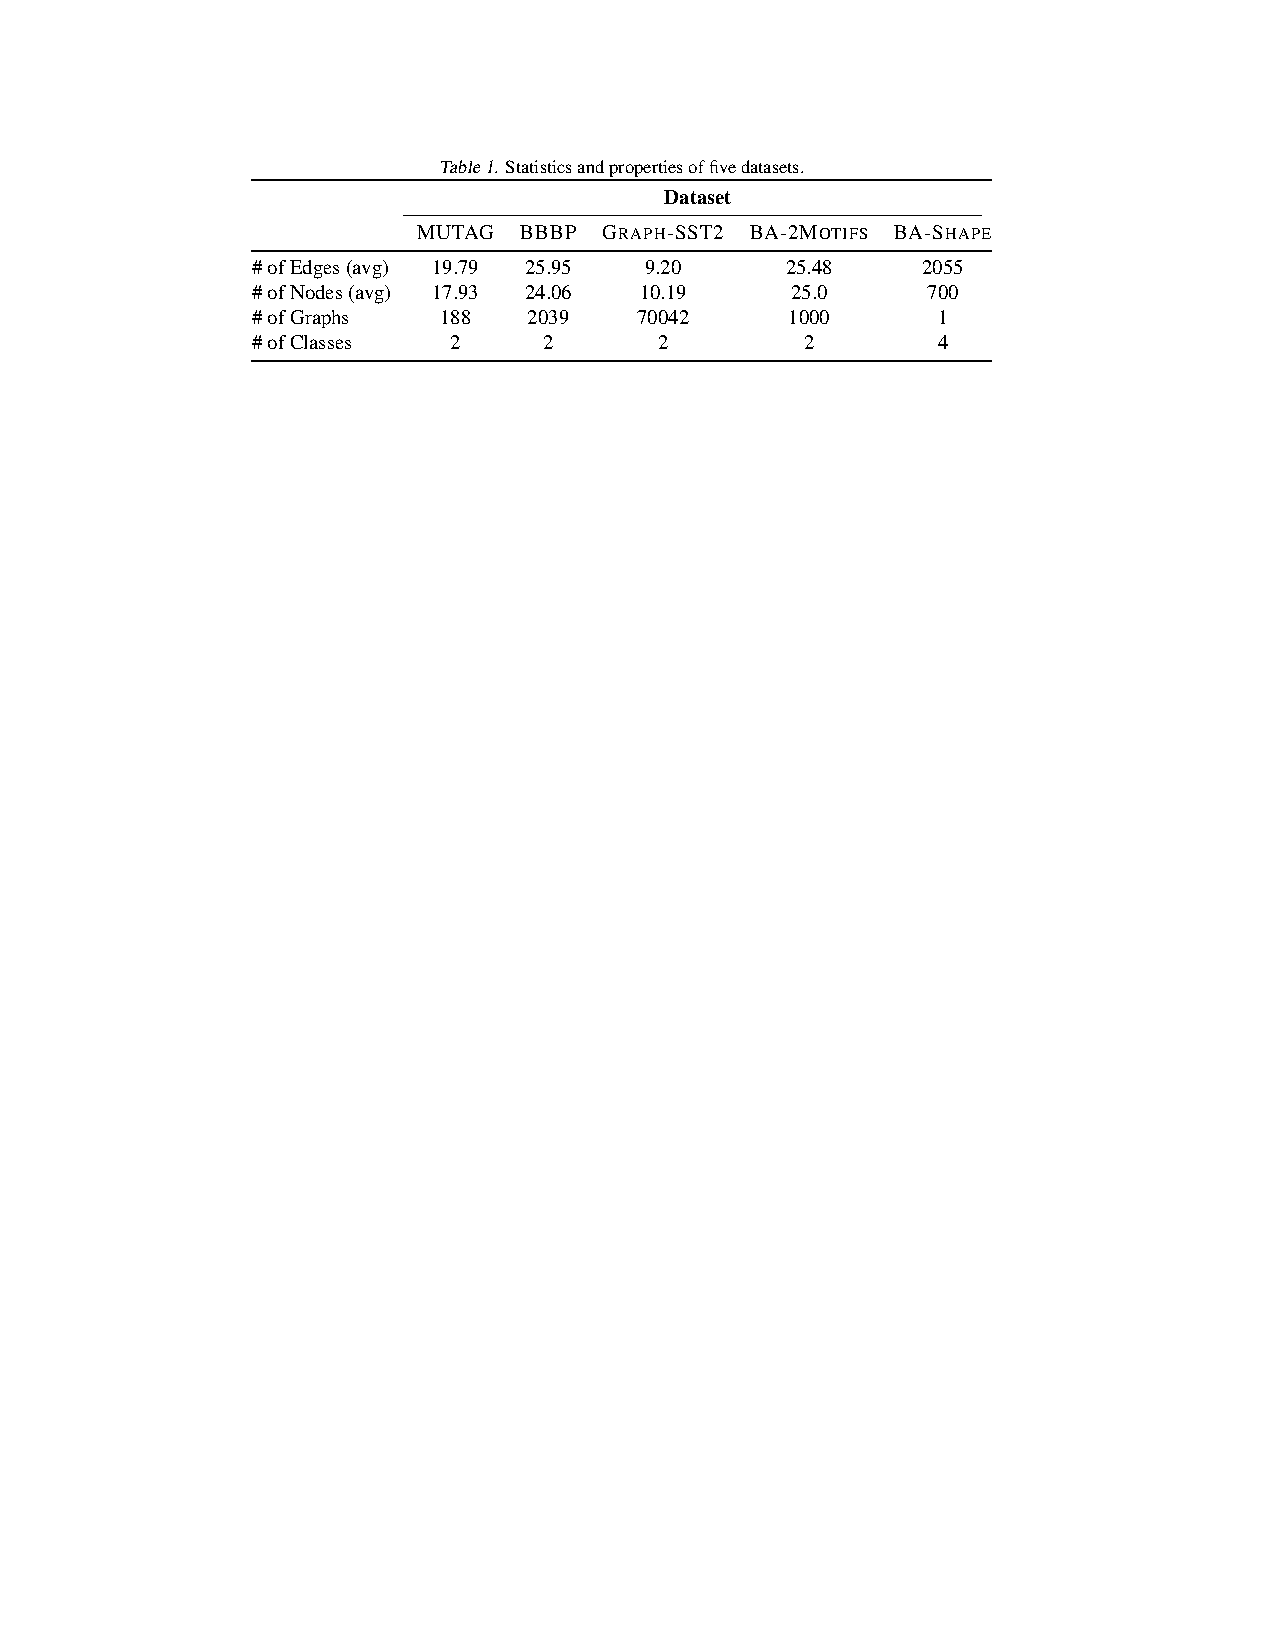
\includegraphics[width=0.8\textwidth]{table1.pdf}
\end{figure*}

我们使用图分类模型作为示例描述了我们提出的 SubgraphX。值得注意的是,我们的 SubgraphX 可以很容易地一般化,用于解释其他任务的图模型,如节点分类和链接预测。对于节点分类模型,解释目标是给定输入图 $\mathcal{G}$ 对单个节点 $v_i$ 的预测。假设 GNN 模型中有 $L$ 层,$v_i$ 的预测仅依赖于其 $L$-hop 计算图,称为 $\mathcal{G}_c$。然后我们的 SubgraphX 不再从输入图 $\mathcal{G}$ 中进行搜索,而是将 $\mathcal{G}_c$ 设置为搜索树根 $\mathcal{N}_0$ 的对应图。此外,在计算边缘贡献时,补零策略应排除目标节点 $v_i$。同时,对于链路预测任务,解释目标为单个链路的预测 $(v_i, v_j)$。那么搜索树的根对应于节点 $v_i$ 和 $v_j$ 的 $L$-hop 计算图。同样,零填充策略在干扰节点特性时忽略 $v_i$ 和 $v_j$。注意,SubgraphX 在解释阶段将 GNN 视为黑盒,只需要访问输入和输出。因此,我们提出的 SubgraphX 可以应用于 GNN 模型的一般家族,包括但不限于GCNs、GATs、GINs 和 Line-Graph NNs。


%%%%%%%%%%%%%%%%%%%%%%%%%%%%%%%%%%%%%%%%%%%%%%%%%%%%%%%%%%%%%%%%%%%%%%
\section{实验研究}\label{sec:Experiment}

\subsection{数据集和实验设置}

我们在不同的数据集和 GNN 模型上进行了广泛的实验,以证明我们提出的方法的有效性。表1报告了数据集的统计信息和属性。我们使用 5 个数据集评估 SubgraphX,用于图分类和节点分类任务,包括合成数据、生物数据和文本数据。我们总结这些数据集如下:

\begin{itemize}
\item MUTAG  和BBBP 是用于图分类任务的分子数据集。在这些数据集中,每个图代表一个分子,而节点是原子,边是键。这些标签是由分子的化学功能决定的。
\item Graph-SST2 是用于图分类的情感图数据集。它使用Biaffine解析器将文本句子转换为图,节点表示单词,边表示单词之间的关系。请注意,节点嵌入被初始化为预先训练的BERT字嵌入。每张图都被其情绪所标记,可以是积极的,也可以是消极的。
\item BA-2Motifs 是一个合成的图分类数据集。每个图包含一个由 Barab´asiAlbert (BA) 模型生成的基于图,它与一个类似房屋的主题或五节点循环主题相连接。这些图表是根据图案的类型进行标记的。所有的节点嵌入都初始化为包含所有1的向量。
\item BA-Shape是一个合成的节点分类数据集。每个图包含一个基本的BA图和几个类似房屋的五节点图案。节点标签由不同节点的成员关系和位置决定。所有的节点嵌入都初始化为包含所有1的向量。
\end{itemize}

我们探索了这些数据集上的三种 GNN 变体,包括 GCNs、GATs 和 GINs。我们实验研究中使用的所有 GNN 模型都经过训练,以获得合理的性能。然后,我们将 SubgraphX 与几个基线进行比较,包括 MCTS GNN、GNNExplainer、PGExplainer。注意 GNNExplainer 和 PGExplainer 代表了最先进的 GNN 解释方法。这里 MCTS GNN 表示使用 MCTS 探索子图,但直接使用这些子图的 GNN 预测作为评分函数的方法。我们谨指出,所有方法都是与公平的设置相比较的。我们使用相同的数字来控制所有方法的解释中的最大节点数。

\begin{figure*}[t]
  \centering
  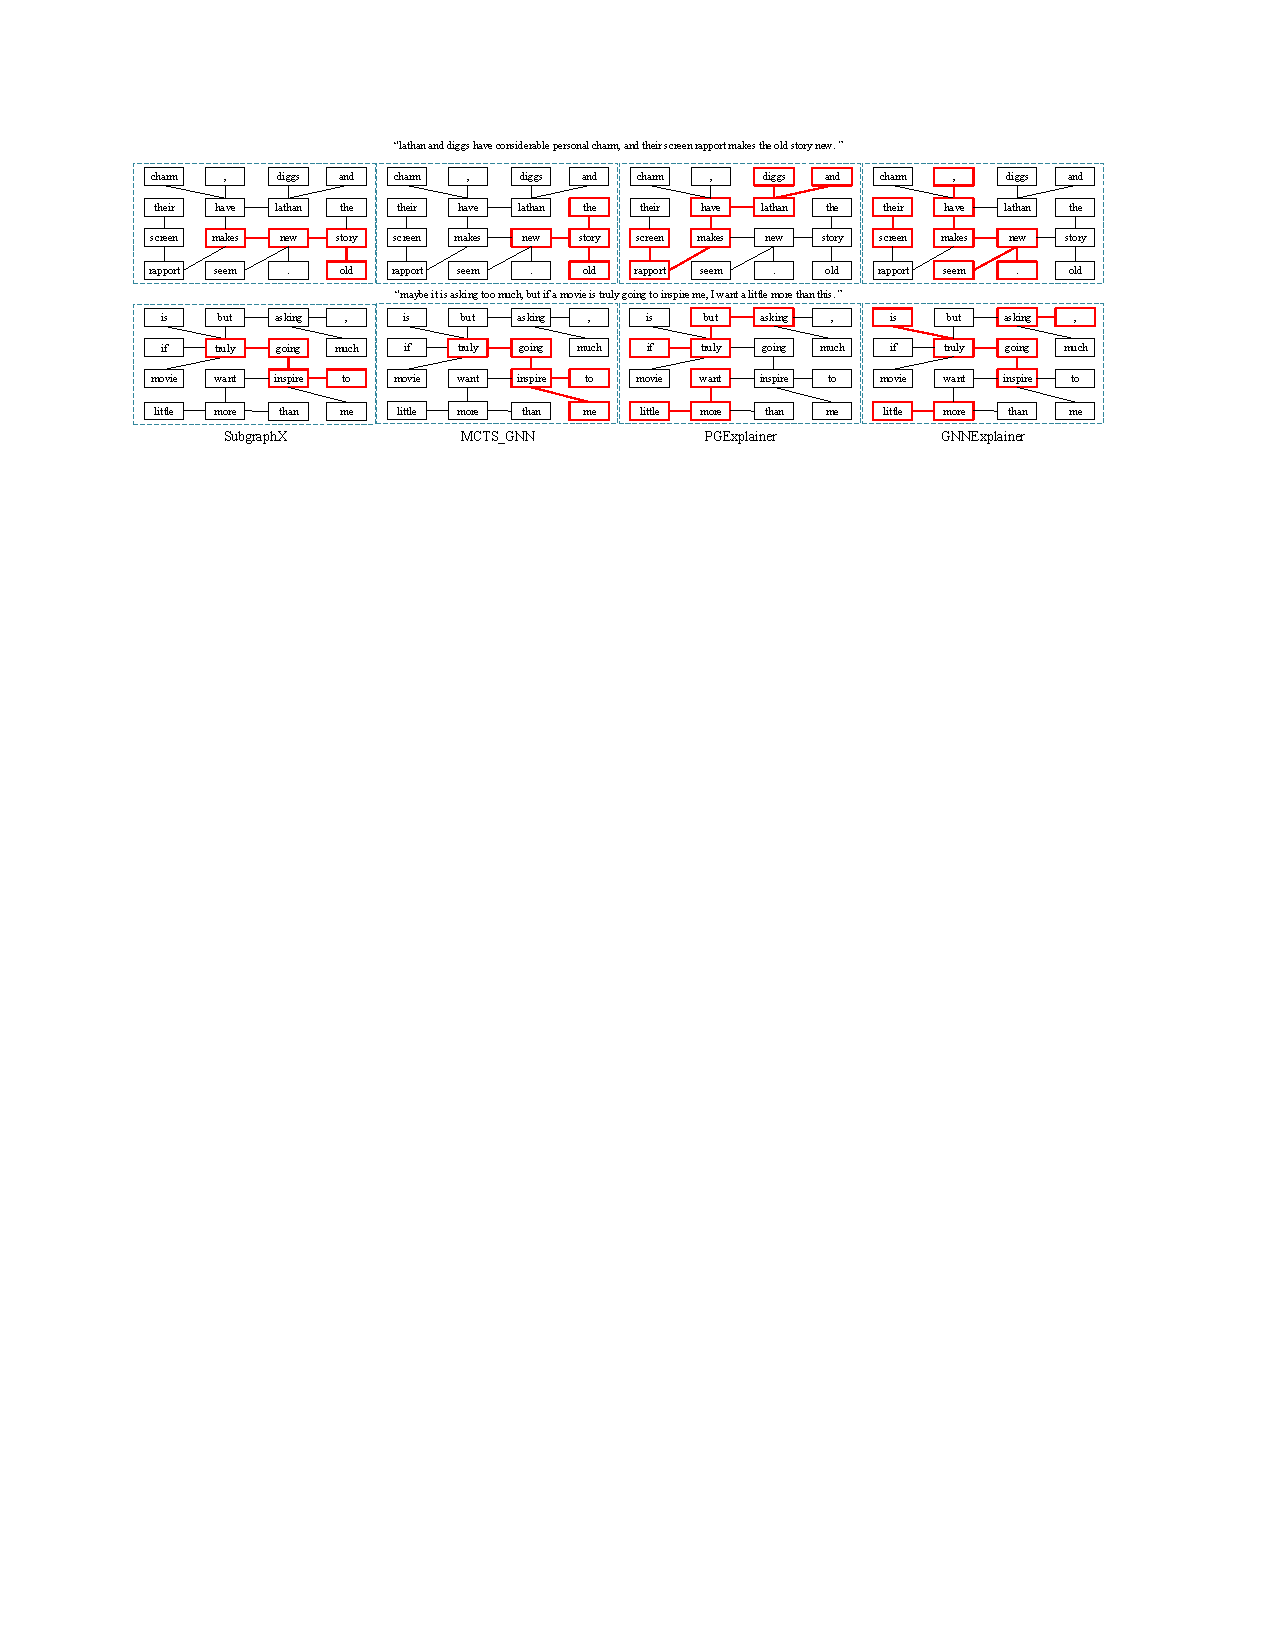
\includegraphics[width=\textwidth]{fig2.pdf}
  \caption{使用 GAT 图分类器对 Graph-SST2 数据集的解释结果。输入的句子显示在解释的顶部。注意,为了简单起见,忽略了一些“不重要”的单词。第一行显示正确预测的解释,第二行报告错误预测的结果。
  }\label{fig:fig2}
\end{figure*}

\begin{figure}[h!]
   \begin{overpic}[width=\columnwidth]{fig3.pdf} \small
   \end{overpic}
   \caption{使用GCN图分类器对BA-2Motifs数据集的解释结果。第一行显示正确预测的解释,第二行报告错误预测的结果。
   }\label{fig:fig3}
\end{figure}

我们在 Intel Xeon Gold 6248 CPU 上使用一个 Nvidia V100 GPU 进行实验。我们的实现基于 Python 3.7.6、PyTorch 1.6.0和 Torch-geometric 1.6.3。对于我们提出的 SubgraphX 和其他具有MCTS的算法,MCTS迭代数M设为20。为了在探索和开发之间找到一个合适的平衡点,我们将Graph- SST2 (GATs)和BBBP (GCNs)模型中的超参数 $\lambda$ 设为5,其他模型中的超参数 $\lambda$ 设为10。由于所有的GNN模型包含 3 个网络层,我们考虑3跳计算图来计算我们的SubgraphX的Shapley值。对于SubgraphX中的蒙特卡罗采样,我们将所有数据集的蒙特卡罗采样步骤T设置为100。对于MCTS†,我们设置蒙特卡罗采样步长为1000,以获得良好的近似值,因为它从图中的所有节点采样。有关数据集、训练过的GNN模型和实验设置的更多细节,请参见补充部分a。我们的代码和数据现在可以在DIG库中公开获得\footnote{\url{https://github.com/divelab/DIG}}。

\begin{figure}[t!]
   \begin{overpic}[width=\columnwidth]{fig4.pdf} \small
   \end{overpic}
   \caption{使用GIN图分类器在MUTAG数据集上解释结果。我们给出了两个正确预测的解释。这里碳、氧和氮分别用黄色、红色和蓝色表示。
   }\label{fig:fig4}
\end{figure}



%%%%%%%%%%%%%%%%%%%%%%%%%%%%%%%%%%%%%%%%%%%%%%%%%%%%%%%%%

\subsection{图分类模型说明}

我们首先使用图分类模型直观地比较SubgraphX和其他基线。结果如图 \ref{fig:fig3}、\ref{fig:fig4} 和 \ref{fig:fig2} 所示,其中重要的子结构以粗体显示。

\begin{figure*}[t]
  \centering
  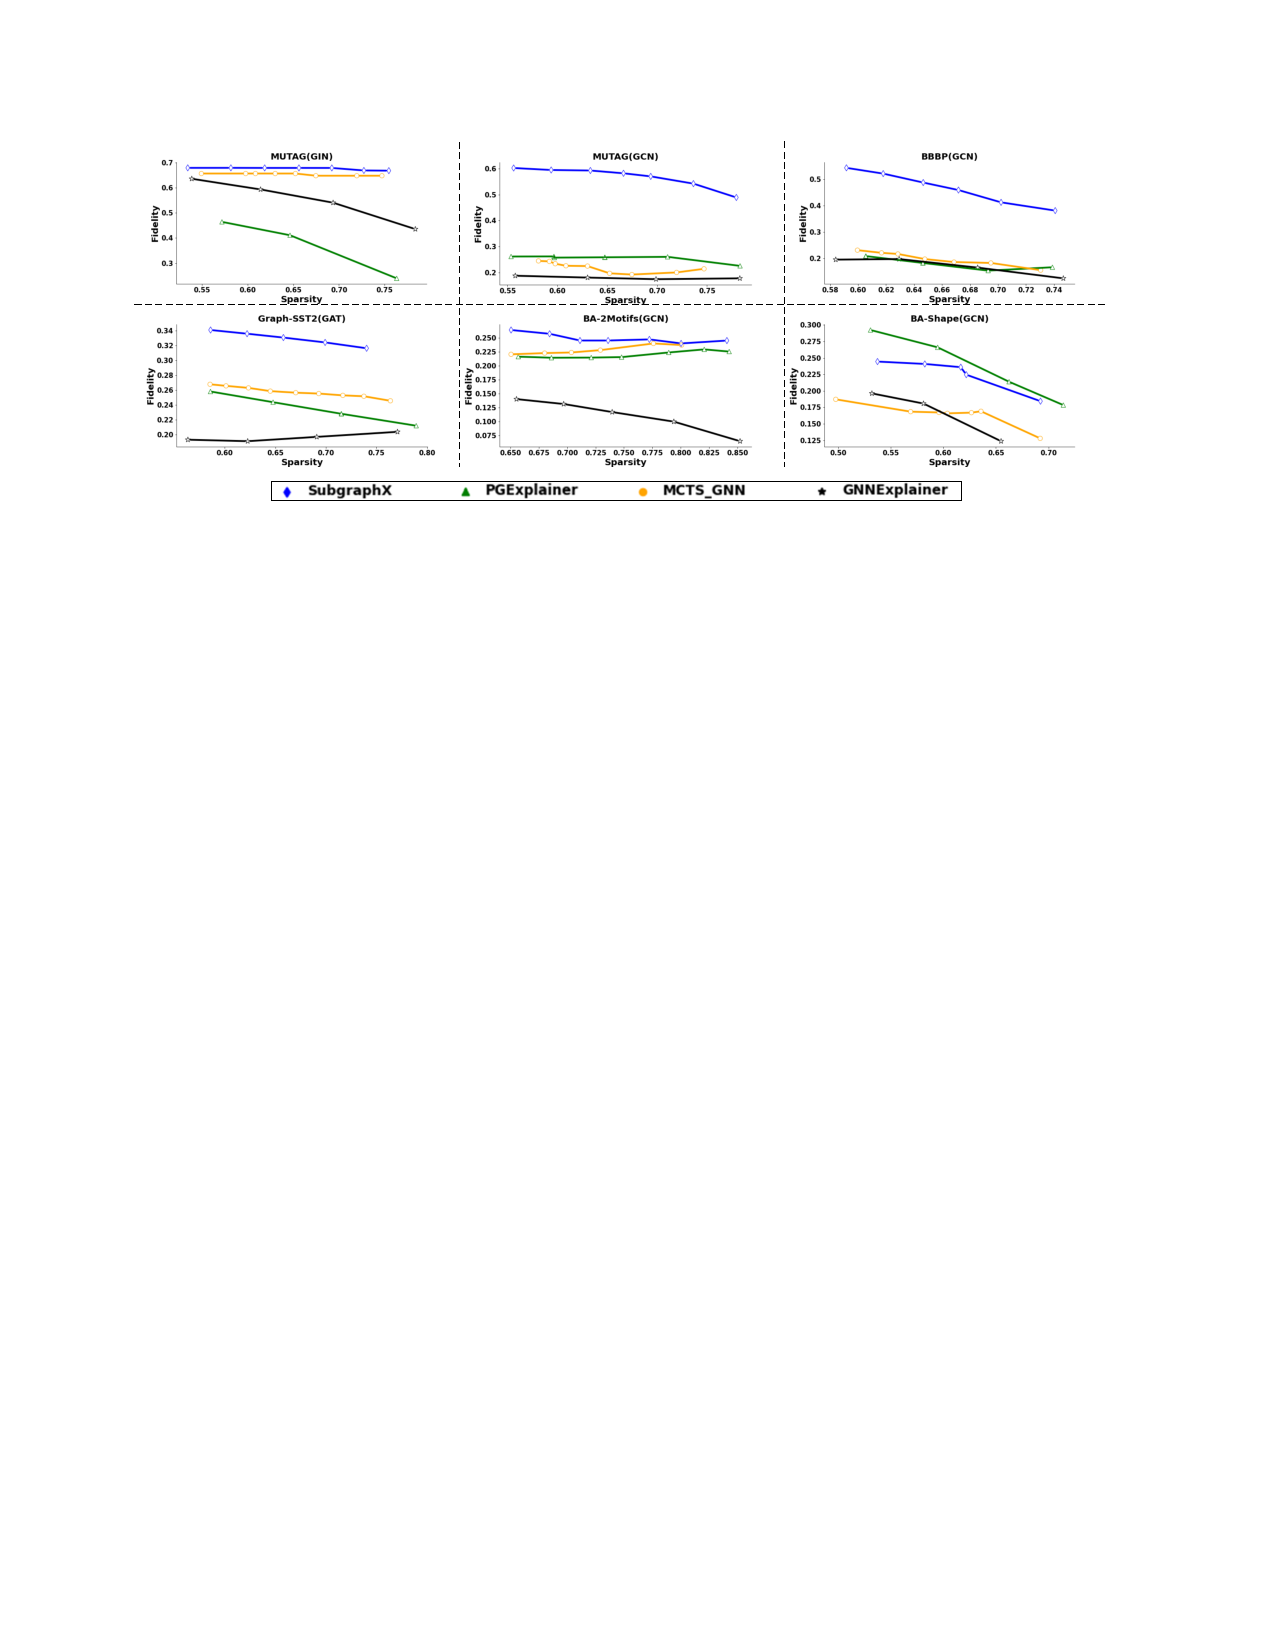
\includegraphics[width=\textwidth]{fig5.pdf}
  \caption{不同解释方法的定量研究。注意,由于稀疏性分数不能完全控制,我们将不同的方法与相似稀疏性水平下的Fidelity分数进行比较。
  }\label{fig:fig5}
\end{figure*}

BA-2Motifs数据集的解释结果如图 \ref{fig:fig3} 所示。我们使用 GCN 作为图分类器,并报告正确和错误预测的解释。由于这是一个综合数据集,我们可以把这些主题看作是解释基础事实的合理近似。在第一行中,模型预测是正确的,我们的 SubgraphX 可以准确地识别出 house-like motif 作为最重要的子图。在第二行中,我们的SubgraphX解释了GNN模型不能捕捉五节点循环 motif 作为重要结构的错误预测,因此预测是错误的。对于这两种情况,我们的SubgraphX可以提供更好的可视化解释,因为我们的方法可以精确地识别能够合理解释预测的简洁子图。此外,我们的解释是连接子图,而PGExplainer和gnexplainer识别离散边。

我们还在图 \ref{fig:fig4} 中展示了MUTAG数据集的解释结果。注意,GINs被用作要解释的图分类模型。由于MUTAG数据集是一个真实的数据集,解释不存在基本事实,因此我们基于化学领域知识评估解释结果。MUTAG中的图是根据对细菌的诱变效应标记的。已知碳环和 $NO_2$ 基团具有诱变作用。我们研究了不同方法提供的解释是否能与化学中发现的碳环和 $NO_2$ 基团相匹配。在这两个例子中,预测都是“诱变的”,我们的SubgraphX成功且准确地将碳环识别为重要的子图。同时,MCTS GNN可以捕获关键子图,但包含多个附加边。PGExplainer和 GNNExplainer的结果仍然包含一些离散的边。

对于数据集 Graph-SST2,我们采用 GATs 作为图模型,报告结果如图 \ref{fig:fig2} 所示。在第一行,预测是正确的,标签是积极的。 我们的SubgraphX和MCTS GNN都能找到具有积极语义的词短语,如“让旧故事变新”,可以合理地解释预测。然而,PGExplainer和 GNNExplainer 提供的解释在语义上不太相关。在第二行,输入是负的,但预测是正的。除了PGExplainer,所有的方法都可以解释GNN模型认为积极短语“真正要启发”是重要的决定,从而产生一个积极但不正确的预测。值得注意的是,我们的方法倾向于包含较少的神经词,如“the”、“me”和“screen”等。

总而言之,我们的SubgraphX可以解释不同图数据和GNN模型的正确和错误预测。我们的解释比比较方法更容易被人理解。图分类模型的更多结果见补充部分B。

\begin{figure}[t!]
   \begin{overpic}[width=\columnwidth]{fig6.pdf} \small
   \end{overpic}
   \caption{对BA-Shape数据集的解释结果。目标节点显示为更大的尺寸。节点标签用不同的颜色表示。
   }\label{fig:fig6}
\end{figure}

%%%%%%%%%%%%%%%%%%%%%%%%%%%%%%%%%%%%%%%%%%%%%

\subsection{节点分类模型说明}

\begin{figure*}[t!]
  \centering
  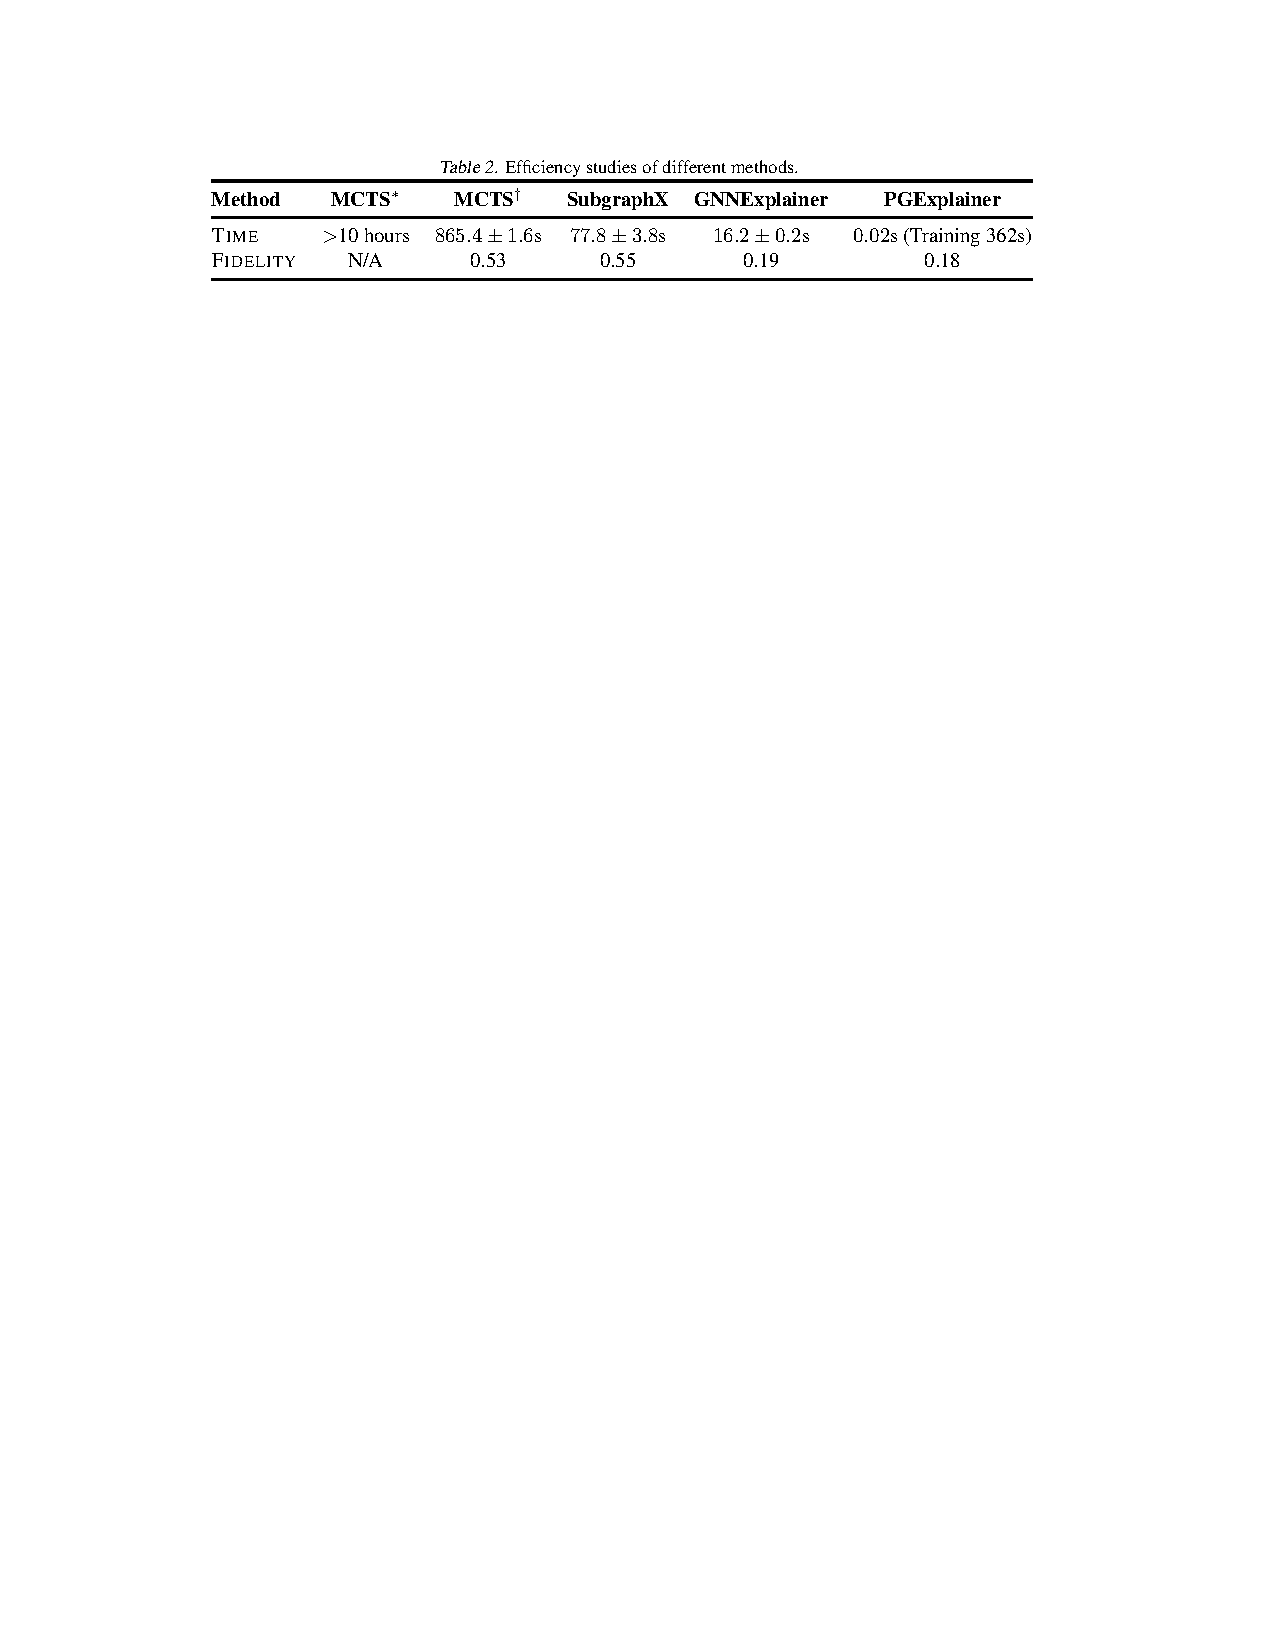
\includegraphics[width=0.8\textwidth]{table2.pdf}
\end{figure*}

我们也比较了不同的方法在节点分类任务。我们使用BA-Shape数据集训练GCN模型来执行节点分类。可视化结果如图 \ref{fig:fig6} 所示,其中重要的子结构以粗体显示。我们可以验证解释是否与标记不同节点的规则(主题)一致。对于这两个示例,都正确地分类了目标节点。显然,我们的SubgraphX正是针对主题作为解释,这是合理的和有希望的。对于其他方法,它们的解释只包括部分母题和其他结构。更多的结果报告在补充部分C。


%%%%%%%%%%%%%%%%%%%%%%%%%%%%%%%%%%%%%%%%%%%%%%%%%%%%

\subsection{定量研究}

虽然可视化对于评估不同的解释方法很重要,但由于缺乏基本事实,人的评估可能不准确。因此,我们进一步进行定量研究,对这些方法进行比较。具体来说,我们采用了保真度和稀疏度指标来评估解释结果。Fidelity度量标准衡量这些解释是否忠实地对模型的预测重要。它从输入图中删除重要的结构,并计算预测之间的差异。此外,稀疏度度量度量的部分结构被确定为重要的解释方法。注意,高稀疏度分数意味着较小的结构被认为是重要的,这可能会影响保真度分数,因为较小的结构(高稀疏度)往往不那么重要(低保真度)。因此,为了进行公平的比较,我们在相似的稀疏性水平下使用Fidelity来比较不同的方法。结果见图 \ref{fig:fig5},其中我们绘制了Fidelity得分相对于稀疏性得分的曲线。显然,在6个实验中,我们提出的方法有5个在不同的稀疏度水平下显著且一致地优于比较方法。对于BAShape (GCN)实验,与PGExplainer相比,我们的SubgraphX获得了稍低但仍然具有竞争力的Fidelity分数。总之,这些结果表明,我们的方法的解释更忠实和重要的GNN模型。评估指标的更多细节在补充部分A中介绍。

%%%%%%%%%%%%%%%%%%%%%%%%%%%%%%%%%%%%%%%%%%%%%%%%%

\subsection{效率研究}

最后,我们研究了所提方法的有效性。对于来自 BBBP 数据集的平均有24.96个节点的50个图,我们展示了获得每个图的解释所需的平均时间成本。实验重复3次,结果见表2。这里的 MCTS∗ 是根据公式(8)计算Shapley值的基线。与我们的SubgraphX相比,不同之处在于使用了蒙特卡罗采样。此外,MCTS†表明,在没有我们提出的近似格式的情况下,用蒙特卡罗采样计算Shapley值的基线。具体地说,MCTS†样本联合集来自于玩家集 $P$ 而不是缩减集 $P^{\prime}$。首先,MCTS* 的时间代价非常高,因为它需要列举所有可能的联合集。接下来,与MCTS†相比,我们的 SubgraphX 快11倍,而得到的解释具有相似的 Fidelity 得分。证明了我们的近似格式是有效和高效的。虽然我们的方法比 GNNExplainer 和 PGExplainer 慢,但是我们的解释的保真度比他们的高出300\%。此外,PGExplainer 需要使用整个数据集来训练它的模型。虽然离线模型训练的成本不能直接进行比较,但当数据集规模较大时,额外的和显著的时间成本可能是一个问题。考虑到我们的解释质量更高,更容易被人理解,我们认为这样的时间复杂度是合理的,可以接受的。

\begin{figure}[t!]
   \centering
   \begin{overpic}[width=0.8\columnwidth]{table3.pdf} \small
   \end{overpic}
\end{figure}

%%%%%%%%%%%%%%%%%%%%%%%%%%%%%%%%%%%%%%%%%%%%%%%%%%%%

\subsection{剪枝研究}

最后,我们讨论了在我们的 MCTS 中的修剪行动。对于与每个非叶树搜索节点相关联的图,我们执行节点剪枝来获得它的子图。具体来说,当一个节点被移除时,所有与它相连的边也被移除。另外,如果移除一个节点后得到多个断开连接的子图,则只保留最大的子图。我们不探索所有可能的节点修剪操作,而是探索两种策略: Low2high和High2low。首先,Low2high根据节点度由低到高排列节点,只考虑前 $k$ 个低度节点对应的剪枝动作。同时High2low将节点从高次到低次进行排序,只考虑前 $k$ 个高次节点进行剪枝。直觉上,High2low更有效,但可能会忽略最优解决方案。在本研究中,我们对BA-Shape(GCNs)采用High2low策略,对其他模型采用Low2high策略,并将所有数据集的 $k$ 设为12。我们通过实验对我们的SubgraphX算法分析了这两种修剪策略,并在表3中显示了平均时间开销和Fidelity评分。具体来说,我们从BBBP数据集中随机选取50个平均节点数为24.96的图,与4.5节相同。另外,我们设置Monte-Carlo采样步长T为100,选取Shapley值最大且节点数小于15的子图计算Fidelity。显然,High2low比Low2high快5倍,但Fidelity得分较低。

%%%%%%%%%%%%%%%%%%%%%%%%%%%%%%%%%%%%%%%%%%%%%%%%%

\section{总结}\label{sec:Conclusion}

虽然已经有相当大的努力致力于研究 GNN 的可解释性,但现有的方法都不能用子图解释GNN的预测。我们认为子图是复杂图的构建块,更容易被人类理解。为此,我们提出SubgraphX通过显式地标识重要的子图来解释GNN。我们采用蒙特卡洛树搜索算法来有效地探索不同的子图。对于每个子图,我们建议通过考虑不同图结构之间的相互作用,使用 Shapley 值来衡量其重要性。为了加快计算速度,我们提出了一种计算Shapley值的有效近似方案,该方案只考虑信息聚集范围内的交互作用。实验结果表明,我们的SubgraphX获得了更高的质量和更容易理解的解释,同时保持时间复杂度可接受。

\paragraph{注:} 可以参考 \url{https://zhuanlan.zhihu.com/p/377245180} 上关于本篇论文的解读。

{\small
\bibliographystyle{ieee}
\bibliography{Saliency}
}

% \end{CJK*}
\end{document}
